\chapter{Node-level (intra-node) analysis}
\label{chapter:node-level}



Once we hit this section, we know that we make no particular good use of our cores.
This is evidenced by the fact that our intra-node scaling is not good (cmp.~Section~\ref{section:high-level:inter-node}), 
i.e.~we measure what we get on one core and then extrapolate what our given number of cores should yield.
But they don't:
The speedup as introduced from \eqref{equation:hpc-terms:speedup} is poor as we increase the core count.
We leave a lot of potential compute capability unused.


Our deep dive starts from an analysis if there is enough concurrency in principle to exploit all cores.
If there are not enough concurrent operations, further analysis is not required. 
The code can be returned immediately to the developers.
Otherwise, we take it from there (Figure~\ref{figure:core:decision-graph}).


%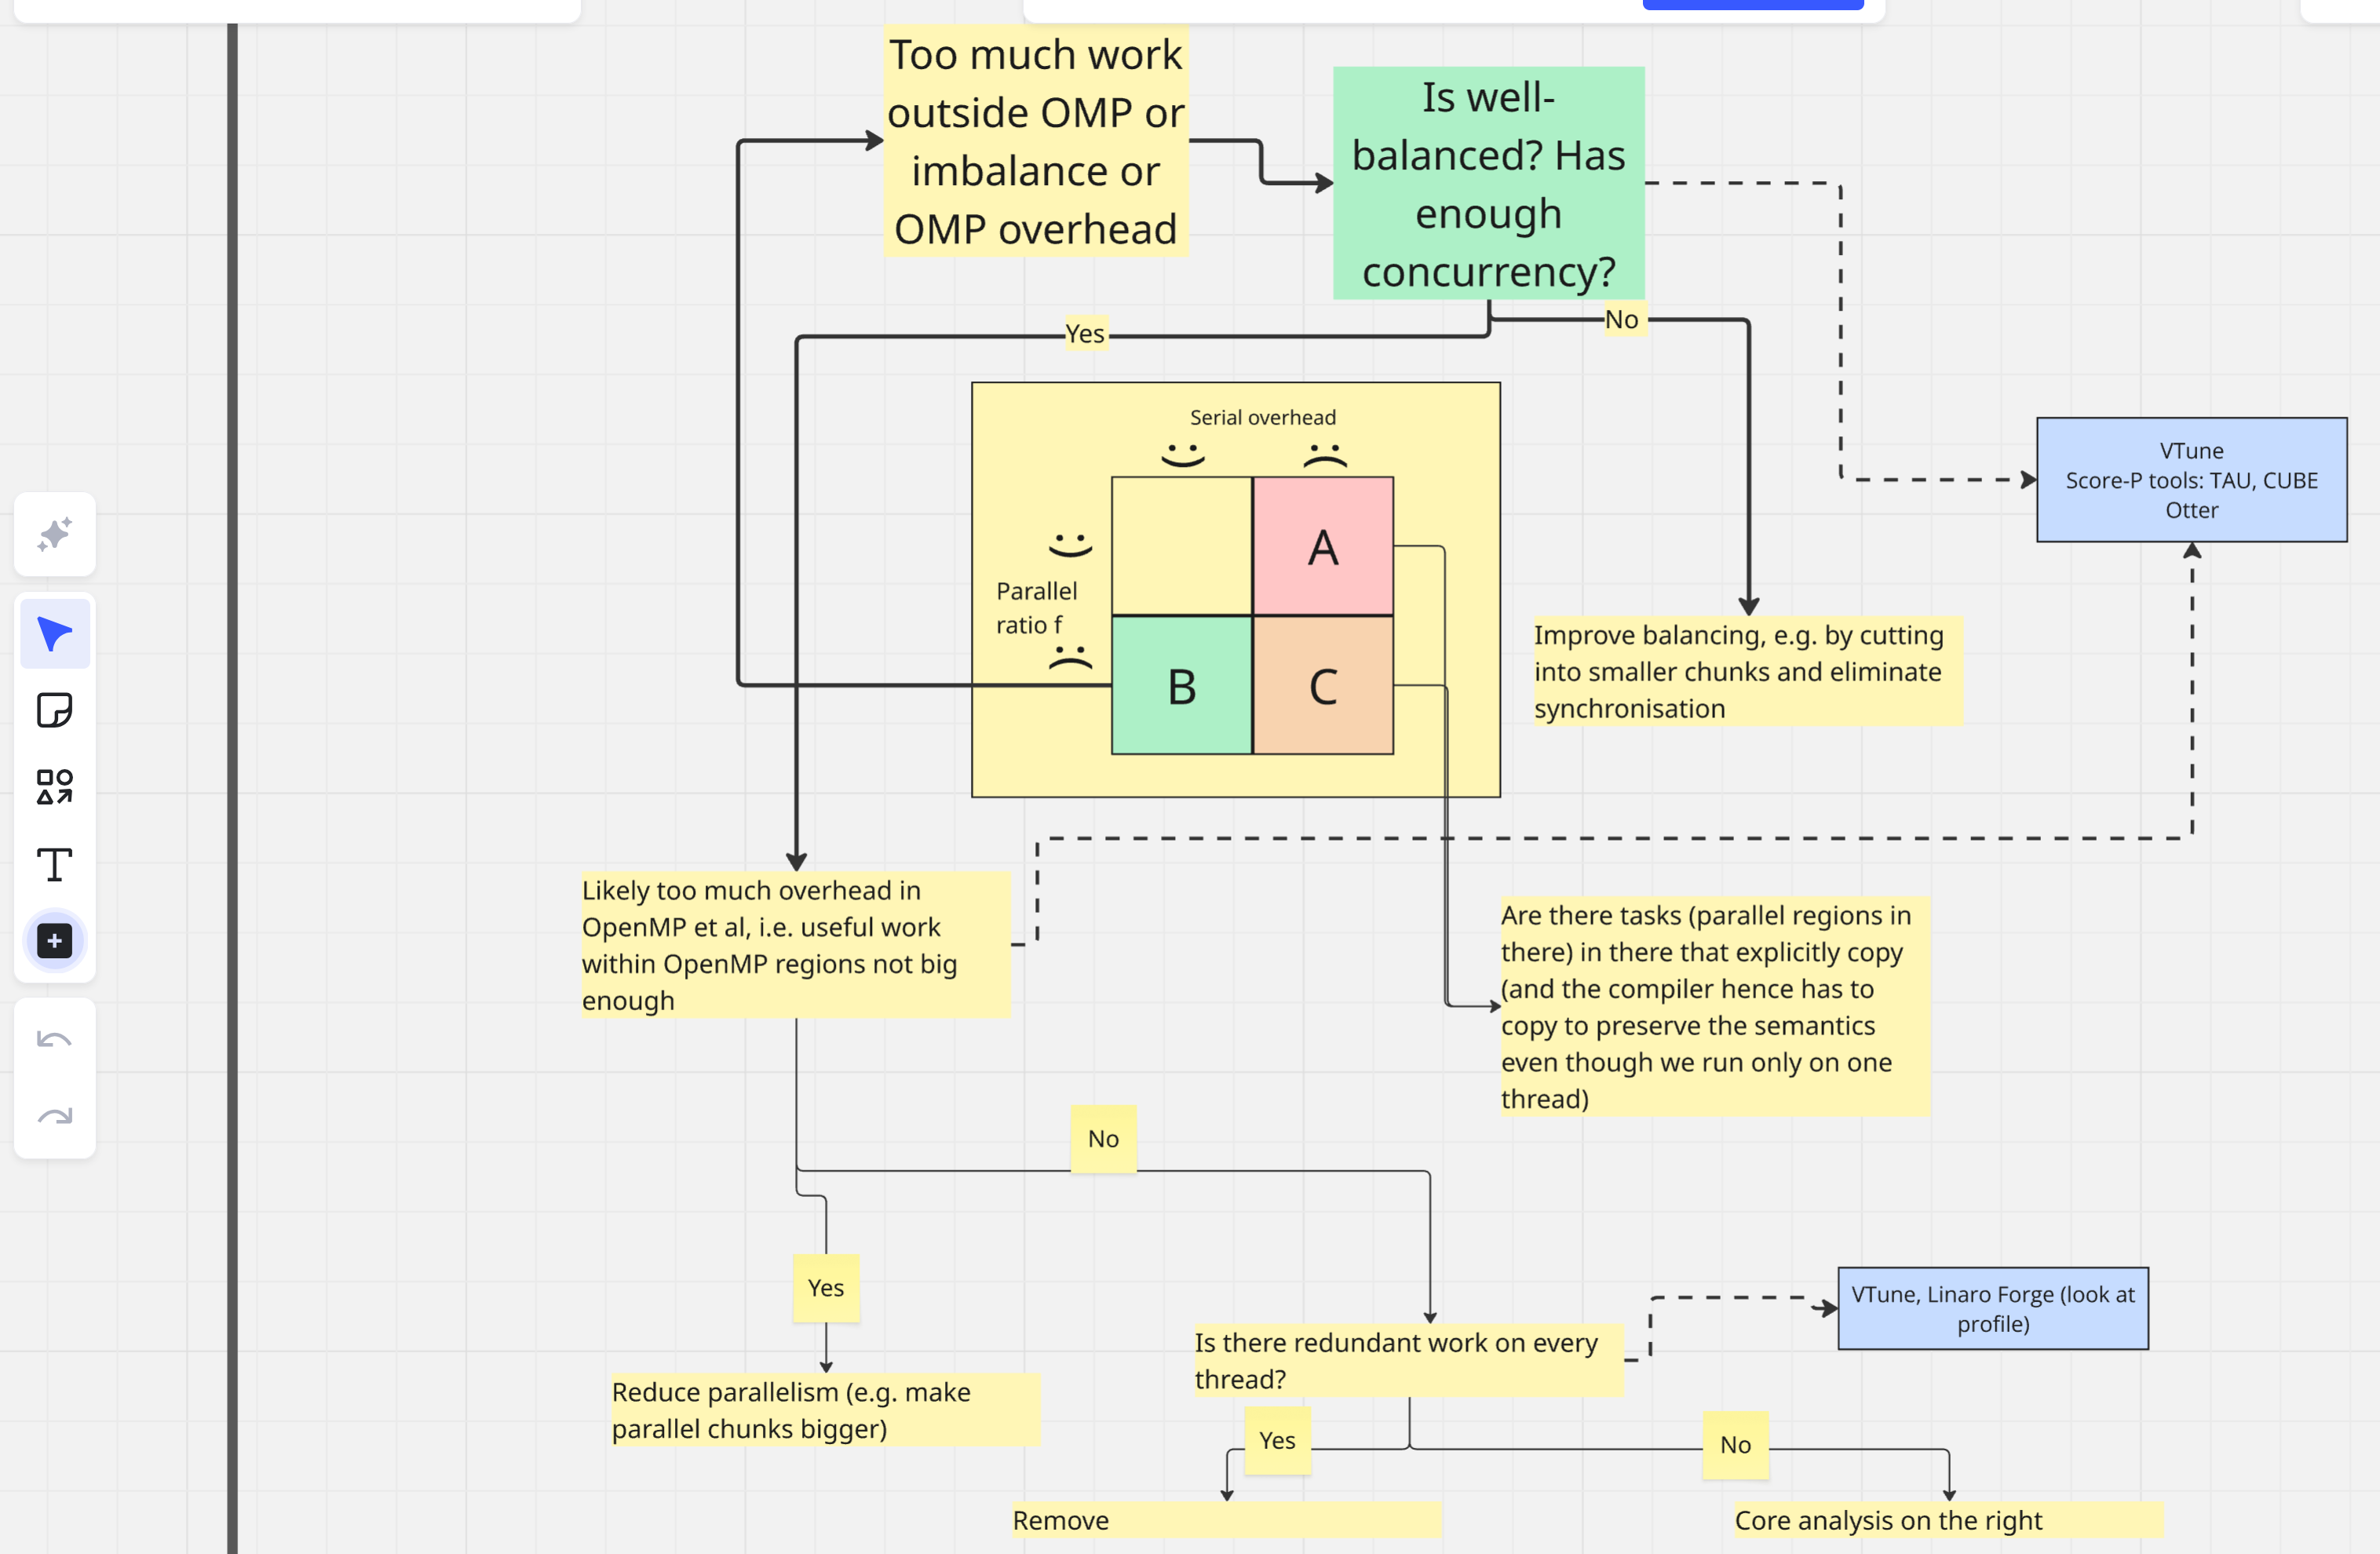
\includegraphics[width=0.8\textwidth]{node-level/whiteboard-intra-node.png}


\subsection*{Preparation}

Inter-node analysis is all about how efficiently we use multiple threads.
Therefore, it focuses predominantly on relative quantities:
How well does the code perform if we add another thread?
However, we cannot study 128+ measurements in one go---even though modern performance analysis tools have quite powerful capabilities to compare different setups.
We need to focus on few setups that yield interesting setup.



\begin{assessmentcrime}
 People study a whole-node run right from the start without a scalability
 analysis beforehand.
\end{assessmentcrime}



\noindent
It makes sense to run a strong scaling test and plot the efficiency. 
Once completed, we can flag those areas where the gradient suddenly changes or   
where the efficiency drops below 80\% or 60\% respectively.
These are the setups (turning points) on which we should focus most of the time.
Do not try to study any other setup, as you'll most likely be swamped with data
that is not relevant or difficult to interpret!

%   \item[$\boxplus$] Use Amdahl's law to characterise your code. If it fits to
%   the law, i.e.~there is an $f_{\text{intra}}$ such that
%   \eqref{equation:amdahl:speedup}.

\paragraph*{How it works}

\begin{itemize}[noitemsep]
  \item[$\boxplus$] Run a strong scaling test and plot the efficiency. Narrow down the number of setups of interest, i.e.~identify regions where the efficiency apruptly changes or falls under a threshold.
\end{itemize}


\paragraph*{How it does not work}

\begin{itemize}[noitemsep]
  \item[$\boxminus$] Start with a full-node run right from the start and hope that you spot interesting trends in the data.
\end{itemize}


\subsection*{Decision graph}


% \begin{figure}[htb]
 \begin{center}
  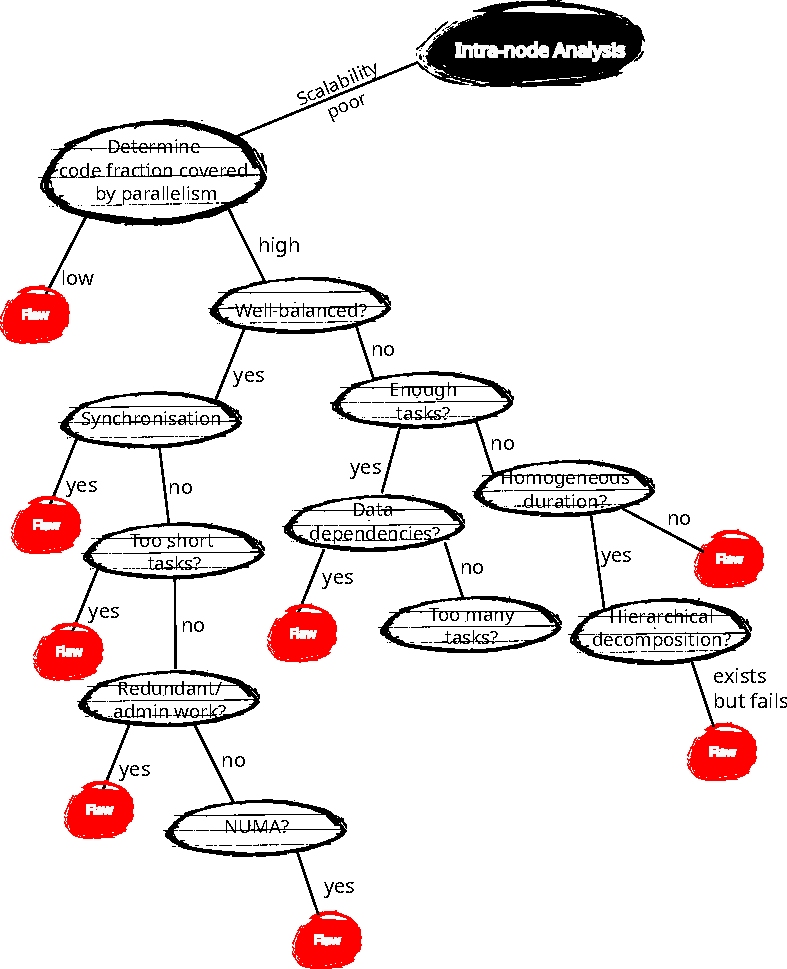
\includegraphics[width=0.65\textwidth]{node-level/decision-graph.pdf}
 \end{center}
%  \caption{
%   Decision graph for inter-node analysis.
%   \label{figure:core:decision-graph}
%  }
% \end{figure}


% \subsection*{Overview}
% 
% 
% \begin{center}
%  \begin{tabular}{p{0.75\textwidth}|r}
%   Flaw & Section \\
%   \hline
%   Determine code fraction covered by parallelism 
%   &
%   \ref{section:node-level:coverage} \\
%   Is the code well-balanced?
%   &
%   \ref{section:node-level:balancing} \\
%   Limited concurrency: Do we have enough tasks?
%   & 
%   \ref{section:node-level:concurrency} \\
%   NUMA effects
%   & 
%   \ref{section:node-level:numa} \\
%   Too small tasks/granularity
%   & 
%   \ref{section:node-level:task-size} \\
%   Synchronisation
%   & 
%   \ref{section:node-level:synchronisation} \\
%   Data dependencies
%   & 
%   \ref{section:node-level:data-dependencies} \\
%   Redundant (administrative) computations
%   & 
%   \ref{section:node-level:redundant-admin} \\
%   Number of tasks
%   & 
%   \ref{section:node-level:task-count} \\
%   Homogeneous task duration
%   & 
%   \ref{section:node-level:homogeneous-duration} \\
%   Can we introduce further hierarchical decomposition?
%   & 
%   \ref{section:node-level:hierarchical-decomposition} \\
%   \hline
%  \end{tabular}
% \end{center}
